\documentclass{standalone}
\usepackage{graphicx}	
\usepackage{amssymb, amsmath, amsthm}
\usepackage{color}

\usepackage{tikz}
\usetikzlibrary{intersections, backgrounds, fadings}

\definecolor{light}{RGB}{220, 188, 188}
\definecolor{mid}{RGB}{185, 124, 124}
\definecolor{dark}{RGB}{143, 39, 39}
\definecolor{highlight}{RGB}{180, 31, 180}
\definecolor{gray10}{gray}{0.1}
\definecolor{gray20}{gray}{0.2}
\definecolor{gray30}{gray}{0.3}
\definecolor{gray40}{gray}{0.4}
\definecolor{gray60}{gray}{0.6}
\definecolor{gray70}{gray}{0.7}
\definecolor{gray80}{gray}{0.8}
\definecolor{gray90}{gray}{0.9}
\definecolor{gray60}{gray}{0.95}

\begin{document}

\begin{tikzpicture}[scale=0.3]
  \pgfmathsetmacro{\dx}{0}
  \pgfmathsetmacro{\dy}{0}
  
  \draw[white] (-17 + \dx, -12 + \dy) rectangle (17 + \dx, 12 + \dy);

  \node[] at (0 + \dx, 9.5 + \dy) { Small $\alpha$, Small $\rho$ };

  \begin{scope}
    \clip (-13 + \dx, -8 + \dy) rectangle (13 + \dx, 8 + \dy);
    \node at (0 + \dx, 0 + \dy) {\includegraphics[width=7.8cm]{gp_low_low.eps}};
  \end{scope}
   
  \draw [->, >=stealth, line width=1] (-13 + \dx, -8 + \dy) -- +(26, 0);
  \draw [->, >=stealth, line width=1] (-13 + \dx, -8.058 + \dy) -- +(0, 16);
  \node[] at (0 + \dx, -10 + \dy) { $x$ };
  \node[] at (-15 + \dx, 0 + \dy) { $f(x)$ };

  \pgfmathsetmacro{\dx}{36}
  \pgfmathsetmacro{\dy}{0}
  
  \draw[white] (-17 + \dx, -12 + \dy) rectangle (17 + \dx, 12 + \dy);

  \node[] at (0 + \dx, 9.5 + \dy) { Medium $\alpha$, Small $\rho$ };

  \begin{scope}
    \clip (-13 + \dx, -8 + \dy) rectangle (13 + \dx, 8 + \dy);
    \node at (0 + \dx, 0 + \dy) {\includegraphics[width=7.8cm]{gp_nom_low.eps}};
  \end{scope}
   
  \draw [->, >=stealth, line width=1] (-13 + \dx, -8 + \dy) -- +(26, 0);
  \draw [->, >=stealth, line width=1] (-13 + \dx, -8.058 + \dy) -- +(0, 16);
  \node[] at (0 + \dx, -10 + \dy) { $x$ };
  \node[] at (-15 + \dx, 0 + \dy) { $f(x)$ };
  
  \pgfmathsetmacro{\dx}{72}
  \pgfmathsetmacro{\dy}{0}
  
  \draw[white] (-17 + \dx, -12 + \dy) rectangle (17 + \dx, 12 + \dy);

  \node[] at (0 + \dx, 9.5 + \dy) { Large $\alpha$, Small $\rho$ };

  \begin{scope}
    \clip (-13 + \dx, -8 + \dy) rectangle (13 + \dx, 8 + \dy);
    \node at (0 + \dx, 0 + \dy) {\includegraphics[width=7.8cm]{gp_high_low.eps}};
  \end{scope}
   
  \draw [->, >=stealth, line width=1] (-13 + \dx, -8 + \dy) -- +(26, 0);
  \draw [->, >=stealth, line width=1] (-13 + \dx, -8.058 + \dy) -- +(0, 16);
  \node[] at (0 + \dx, -10 + \dy) { $x$ };
  \node[] at (-15 + \dx, 0 + \dy) { $f(x)$ };



  \pgfmathsetmacro{\dx}{0}
  \pgfmathsetmacro{\dy}{-24}
  
  \draw[white] (-17 + \dx, -12 + \dy) rectangle (17 + \dx, 12 + \dy);

  \node[] at (0 + \dx, 9.5 + \dy) { Small $\alpha$, Medium $\rho$ };

  \begin{scope}
    \clip (-13 + \dx, -8 + \dy) rectangle (13 + \dx, 8 + \dy);
    \node at (0 + \dx, 0 + \dy) {\includegraphics[width=7.8cm]{gp_low_nom.eps}};
  \end{scope}
   
  \draw [->, >=stealth, line width=1] (-13 + \dx, -8 + \dy) -- +(26, 0);
  \draw [->, >=stealth, line width=1] (-13 + \dx, -8.058 + \dy) -- +(0, 16);
  \node[] at (0 + \dx, -10 + \dy) { $x$ };
  \node[] at (-15 + \dx, 0 + \dy) { $f(x)$ };

  \pgfmathsetmacro{\dx}{36}
  \pgfmathsetmacro{\dy}{-24}
  
  \draw[white] (-17 + \dx, -12 + \dy) rectangle (17 + \dx, 12 + \dy);

  \node[] at (0 + \dx, 9.5 + \dy) { Medium $\alpha$, Medium $\rho$ };

  \begin{scope}
    \clip (-13 + \dx, -8 + \dy) rectangle (13 + \dx, 8 + \dy);
    \node at (0 + \dx, 0 + \dy) {\includegraphics[width=7.8cm]{gp_nom_nom.eps}};
  \end{scope}
   
  \draw [->, >=stealth, line width=1] (-13 + \dx, -8 + \dy) -- +(26, 0);
  \draw [->, >=stealth, line width=1] (-13 + \dx, -8.058 + \dy) -- +(0, 16);
  \node[] at (0 + \dx, -10 + \dy) { $x$ };
  \node[] at (-15 + \dx, 0 + \dy) { $f(x)$ };
  
  \pgfmathsetmacro{\dx}{72}
  \pgfmathsetmacro{\dy}{-24}
  
  \draw[white] (-17 + \dx, -12 + \dy) rectangle (17 + \dx, 12 + \dy);

  \node[] at (0 + \dx, 9.5 + \dy) { Large $\alpha$, Medium $\rho$ };

  \begin{scope}
    \clip (-13 + \dx, -8 + \dy) rectangle (13 + \dx, 8 + \dy);
    \node at (0 + \dx, 0 + \dy) {\includegraphics[width=7.8cm]{gp_high_nom.eps}};
  \end{scope}
   
  \draw [->, >=stealth, line width=1] (-13 + \dx, -8 + \dy) -- +(26, 0);
  \draw [->, >=stealth, line width=1] (-13 + \dx, -8.058 + \dy) -- +(0, 16);
  \node[] at (0 + \dx, -10 + \dy) { $x$ };
  \node[] at (-15 + \dx, 0 + \dy) { $f(x)$ };
 
 
 
  \pgfmathsetmacro{\dx}{0}
  \pgfmathsetmacro{\dy}{-48}
  
  \draw[white] (-17 + \dx, -12 + \dy) rectangle (17 + \dx, 12 + \dy);

  \node[] at (0 + \dx, 9.5 + \dy) { Small $\alpha$, Large $\rho$ };

  \begin{scope}
    \clip (-13 + \dx, -8 + \dy) rectangle (13 + \dx, 8 + \dy);
    \node at (0 + \dx, 0 + \dy) {\includegraphics[width=7.8cm]{gp_low_high.eps}};
  \end{scope}
   
  \draw [->, >=stealth, line width=1] (-13 + \dx, -8 + \dy) -- +(26, 0);
  \draw [->, >=stealth, line width=1] (-13 + \dx, -8.058 + \dy) -- +(0, 16);
  \node[] at (0 + \dx, -10 + \dy) { $x$ };
  \node[] at (-15 + \dx, 0 + \dy) { $f(x)$ };

  \pgfmathsetmacro{\dx}{36}
  \pgfmathsetmacro{\dy}{-48}
  
  \draw[white] (-17 + \dx, -12 + \dy) rectangle (17 + \dx, 12 + \dy);

  \node[] at (0 + \dx, 9.5 + \dy) { Medium $\alpha$, Large $\rho$ };

  \begin{scope}
    \clip (-13 + \dx, -8 + \dy) rectangle (13 + \dx, 8 + \dy);
    \node at (0 + \dx, 0 + \dy) {\includegraphics[width=7.8cm]{gp_nom_high.eps}};
  \end{scope}
   
  \draw [->, >=stealth, line width=1] (-13 + \dx, -8 + \dy) -- +(26, 0);
  \draw [->, >=stealth, line width=1] (-13 + \dx, -8.058 + \dy) -- +(0, 16);
  \node[] at (0 + \dx, -10 + \dy) { $x$ };
  \node[] at (-15 + \dx, 0 + \dy) { $f(x)$ };
  
  \pgfmathsetmacro{\dx}{72}
  \pgfmathsetmacro{\dy}{-48}
  
  \draw[white] (-17 + \dx, -12 + \dy) rectangle (17 + \dx, 12 + \dy);

  \node[] at (0 + \dx, 9.5 + \dy) { Large $\alpha$, Large $\rho$ };

  \begin{scope}
    \clip (-13 + \dx, -8 + \dy) rectangle (13 + \dx, 8 + \dy);
    \node at (0 + \dx, 0 + \dy) {\includegraphics[width=7.8cm]{gp_high_high.eps}};
  \end{scope}
   
  \draw [->, >=stealth, line width=1] (-13 + \dx, -8 + \dy) -- +(26, 0);
  \draw [->, >=stealth, line width=1] (-13 + \dx, -8.058 + \dy) -- +(0, 16);
  \node[] at (0 + \dx, -10 + \dy) { $x$ };
  \node[] at (-15 + \dx, 0 + \dy) { $f(x)$ };
 
\end{tikzpicture}

\end{document}  